\documentclass{beamer}

\mode<presentation>
{
  %\usetheme{CambridgeUS}
  %\usetheme{Frankfurt}
  \usetheme{Singapore}
  %\usecolortheme{crane}
  \usefonttheme{professionalfonts}
  %\usefonttheme[onlymath]{serif}
  
  \setbeamertemplate{blocks}[rounded][shadow=true]
}

\usepackage{pgfpages}

\usepackage{alltt,verbatim,amsmath,times,empheq}
\usepackage{bm}
\usepackage[english]{babel}
\usepackage[utf8]{inputenc}

%\usepackage{times}
%\usepackage[T1]{fontenc}
% Or whatever. Note that the encoding and the font should match. If T1
% does not look nice, try deleting the line with the fontenc.

%\usepackage{hyperref}

\usepackage{multimedia,xmpmulti}

\usepackage{animate}

\definecolor{dark red}{HTML}{E41A1C}
\definecolor{dark green}{HTML}{4DAF4A}
\definecolor{dark violet}{HTML}{984EA3}
\definecolor{dark blue}{HTML}{084594}
\definecolor{dark orange}{HTML}{FF7F00}
\definecolor{light blue}{HTML}{377EB8}
\definecolor{light red}{HTML}{FB9A99}
\definecolor{light violet}{HTML}{CAB2D6}

\setbeamercolor{boxed}{fg=black,bg=uaf yellow}

\newcommand{\CC}{\mathbb{C}}
\newcommand{\NN}{\mathbb{N}}
\newcommand{\RR}{\mathbb{R}}
\newcommand{\ZZ}{\mathbb{Z}}
\newcommand{\Acal}{\mathcal{A}}
\newcommand{\Bcal}{\mathcal{B}}
\newcommand{\Ccal}{\mathcal{C}}
\newcommand{\Ncal}{\mathcal{N}}
\newcommand{\Kcal}{\mathcal{K}}

\newcommand{\bF}{\mathbf{F}}
\newcommand{\bQ}{\mathbf{Q}}
\newcommand{\bU}{\mathbf{U}}
\newcommand{\bbU}{\bar{\bU}}
\newcommand{\bu}{\mathbf{u}}
\newcommand{\bv}{\mathbf{v}}
\newcommand{\bx}{\mathbf{x}}

\newcommand{\Div}{\nabla\cdot}
\newcommand{\eps}{\epsilon}
\newcommand{\grad}{\nabla}
\newcommand{\lap}{\triangle}
\DeclareMathOperator{\trace}{tr}
\renewcommand{\bar}{\overline}

\newcommand{\ddx}[1]{\frac{\partial #1}{\partial x}}
\newcommand{\ddy}[1]{\frac{\partial #1}{\partial y}}
\newcommand{\pp}[2]{\frac{\partial #1}{\partial #2}}
\newcommand{\ppt}[1]{\frac{\partial #1}{\partial t}}
\newcommand{\ppT}[1]{\frac{\partial #1}{\partial T}}
\newcommand{\ppx}[1]{\frac{\partial #1}{\partial x}}
\newcommand{\ppy}[1]{\frac{\partial #1}{\partial y}}
\newcommand{\ppz}[1]{\frac{\partial #1}{\partial z}}
\newcommand{\ppxx}[1]{\frac{\partial^2 #1}{\partial x^2}}
\newcommand{\ppzz}[1]{\frac{\partial^2 #1}{\partial z^2}}

\newcommand{\Tnorm}[1]{\left|\!\left|\!\left|#1\right|\!\right|\!\right|}
\newcommand{\rhow}{\rho_{\text{w}}}
\newcommand{\Wq}{W^{1,q}(\Omega)}
\newcommand{\half}{\frac12}

%\setbeamercolor{redtext}{fg=red!80!black}
\setbeamercolor{redtext}{fg=red!94!black}
%\setbeamercolor{greentext}{fg=green!80!black}
\setbeamercolor{greentext}{fg=green!60!black}
%\setbeamercolor{bluetext}{fg=blue!70!black}
\setbeamercolor{bluetext}{fg=blue!90!black}
\setbeamercolor{yellowtext}{fg=yellow!95!black}
\setbeamercolor{orangetext}{fg=yellow!50!red}

\newcommand{\green}{\usebeamercolor[fg]{greentext}}
\newcommand{\blue}{\usebeamercolor[fg]{bluetext}}
\newcommand{\red}{\usebeamercolor[fg]{redtext}}

\renewcommand{\L}{\emph{Left}}
\newcommand{\R}{\emph{Right}}



\title[what is a variational inequality]{What is a \emph{variational inequality}?}

\author[Bueler]{Ed Bueler}

\institute[UAF]{
  \tiny Dept of Mathematics and Statistics and Geophysical Institute \\

  University of Alaska Fairbanks
}

\date{\tiny 23 January, 2014}


\setbeamerfont{date}{size=\scriptsize}

\subject{variational inequality}


%\begin{comment}
\AtBeginSection[]
{
  \begin{frame}<beamer>
    \frametitle{Outline}
    \tableofcontents[currentsection,hideallsubsections]
  \end{frame}
}
%\end{comment}


\begin{document}
\graphicspath{{../commonfigs/}}

\begin{frame}
  \titlepage
\end{frame}


% NO OUTLINE BECAUSE ONE APPEARS AT START OF EACH SECTION:
%\begin{comment}
\begin{frame}
  \frametitle{Outline}
  \tableofcontents[hideallsubsections]
  % You might wish to add the option [pausesections]
\end{frame}
%\end{comment}


\section[problems]{problems you can write as variational inequalities}



\begin{frame}
  \frametitle{functional and convex set}

$$J[v] = \int_0^L \frac{1}{2} (v')^2 - f v$$

$$\mathcal{K} = \left\{v \in H_0^1 \,:\, v \ge \psi\right\}$$
\end{frame}


\begin{frame}
  \frametitle{convexity}

if $u\in \mathcal{K}$ is minimizer and if $v\in\mathcal{K}$ and if $0\le \eps \le 1$ then

$(1 - \eps) u + \eps v = u + \eps (v-u) \in \mathcal{K}$ because $\mathcal{K}$ is convex 

\vspace{0.5in}

FIXME: picture first as linear combination

\vspace{0.5in}

FIXME: ... then as vector directed from base $u$
\end{frame}


\begin{frame}
  \frametitle{first variation calculation}

if $u\in \mathcal{K}$ is minimizer and if $v\in\mathcal{K}$ and if $0\le \eps \le 1$ then
   \begin{align*}
   0 &\le J[u + \eps(v-u)] - J[u] \\
     &= \int_0^L \frac{1}{2} \left[(u'+\eps (v-u)')^2-(u')^2\right] - f \left(u+\eps(v-u) - u\right) \\
     &= \int_0^L \frac{1}{2} \left[(u')^2+ 2 \eps u' (v'-u') + \eps^2 (v'-u')^2 - (u')^2\right] - f \eps(v-u) \\
     &= \eps \int_0^L u' (v'-u') - f (v-u) + \eps^2 \int_0^L (v'-u')^2
   \end{align*}
\end{frame}


\begin{frame}
  \frametitle{whence the variational inequality}

\begin{itemize}
\item so far: if $0<\eps\le 1$
\begin{align*}
0 &\le \frac{J[u + \eps(v-u)] - J[u]}{\eps} \\
  &= \int_0^L u' (v'-u') - f (v-u) + \eps \int_0^L (v'-u')^2
\end{align*}
\item \emph{thus} as $\eps \to 0$, we know that $u\in\mathcal{K}$ satisfies
  $$\int_0^L u' (v'-u') - f (v-u) \ge 0 \qquad \forall v\in\mathcal{K}$$
\end{itemize}
\end{frame}


\begin{frame}
  \frametitle{FIXME}

\end{frame}


\begin{frame}
  \frametitle{FIXME}

\end{frame}


\begin{frame}
  \frametitle{FIXME}

\end{frame}


\begin{frame}
  \frametitle{FIXME}

\end{frame}


\begin{frame}
  \frametitle{the 3-point case of obstacle problem, pictured}

\begin{columns}
\begin{column}{0.5\textwidth}
\begin{center}
%\includegraphics[width=1.0\textwidth]{oned-basecase}
\end{center}
\end{column}
\begin{column}{0.5\textwidth}
\begin{center}
FIXME: show three-axis view of same thing here
\end{center}
\end{column}
\end{columns}
\end{frame}


\begin{frame}
  \frametitle{convex set and solution of variational inequality}

\begin{center}
%\includegraphics[width=0.65\textwidth]{convexvar}
\end{center}
\end{frame}





\begin{frame}
  \frametitle{SIA: weak formulation = variational inequality} 

\begin{itemize}
\item issue: SIA equation applies only on domain where $s>b \iff h > 0$
\item the change $h \to u$ transforms  constraint $s \ge b$ into $u \ge 0$
\item define convex constraint set
  $$\Kcal := \{ v \in W^{1,p}_0 (\Omega), v \ge 0 \}$$
\end{itemize}

\begin{block}{definition} 
$u \in \Kcal$ solves the \emph{steady shallow ice sheet problem} if
\begin{align*}
\int_{\Omega}    \left( \mu  | \nabla u - \Phi(u) |^{p-2} 
( \nabla u - \Phi(u) )    \right)  \cdot \nabla ( v - u )  
\ge \int_{\Omega} \alpha(u) (  v -  u ) 
\end{align*}
for all $v \in \Kcal$ \hfill \scriptsize (Jouvet-Bueler 2012)
\end{block}
\end{frame}


\begin{frame}
  \frametitle{SIA: an analogy}

\begin{columns}
\begin{column}{0.35\textwidth}
\begin{itemize}
\item ice sheet surface \\ = \alert{membrane}
\item bedrock = \alert{obstacle}
\end{itemize}
\vfill
\begin{center}
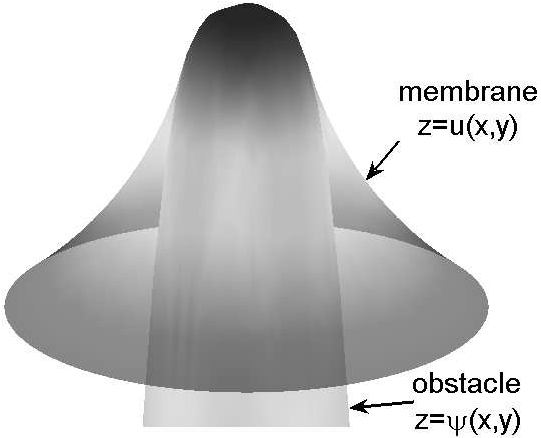
\includegraphics[width=1.1\textwidth]{classicalobs}
\end{center}
\end{column}
\begin{column}{0.65\textwidth}
\begin{center}
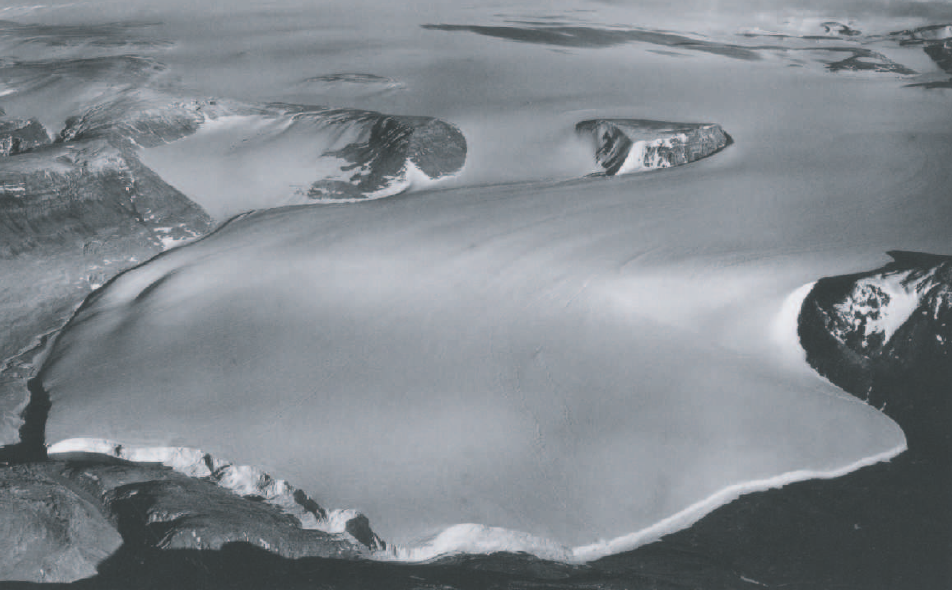
\includegraphics[width=0.8\textwidth]{polaris} \\
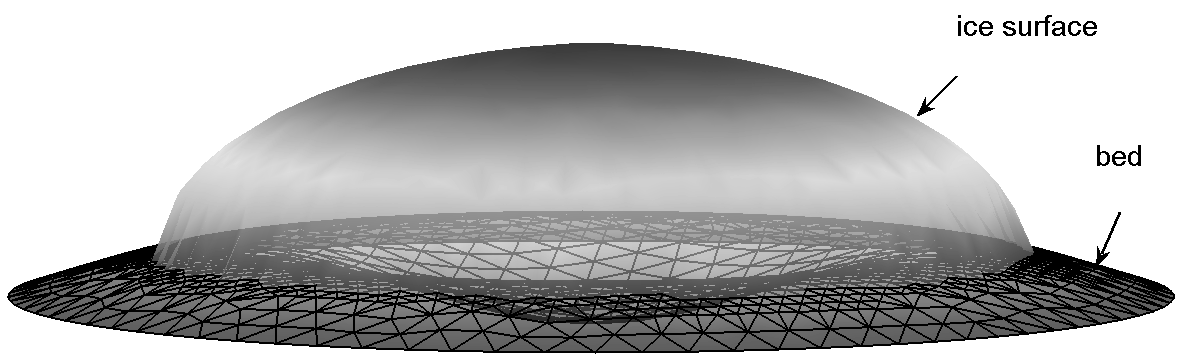
\includegraphics[width=\textwidth]{capnonflatobs}
\end{center}
\end{column}
\end{columns}
\end{frame}


\begin{frame}
  \frametitle{existence and uniqueness for a restricted problem} 

\begin{block}{(easy) theorem}
if $\alpha,\Phi$ were independent of $u$ then the variational inequality is equivalent to:

\begin{equation*}
u \text{ minimizes} \qquad J(v) = \frac{\mu}{p} \int_{\Omega} |\nabla v - \Phi |^p - \int_{\Omega}  \alpha v
\end{equation*}

over $v\in\mathcal{K}$; this admits a unique solution \hfill \scriptsize (Jouvet-Bueler 2012)
\end{block}

\bigskip
\begin{itemize}
\item gives ice sheet existence and uniqueness only if
  \begin{itemize}
  \item[$\circ$]  bedrock is flat ($\Phi = 0$) and
  \item[$\circ$]  mass balance is elevation-independent ($a=a(x,y)$)
  \end{itemize}
\item but otherwise: $\alpha,\Phi$ are not independent of $u$
\end{itemize}
\end{frame}
 

\begin{frame} 
  \frametitle{ existence in the general case } 

\begin{itemize}
\item $p>2$ so $W^{1,p}_0 (\Omega) \hookrightarrow C(\overline{\Omega})$
\item define map $\mathcal{A}:C(\overline{\Omega}) \rightarrow C(\overline{\Omega})$,
which takes $w$ to the unique $u$ solving (over $v\in \mathcal{K}$)
\begin{align*}
\int_{\Omega}   \mu  \left( | \nabla u - \Phi(w) |^{p-2} 
( \nabla u - \Phi(w) )    \right)  \cdot \nabla ( v - u )  
\ge \int_{\Omega} \alpha(w) (  v -  u )
\end{align*}
\end{itemize}

\begin{block}{result}
the map $\mathcal{A}$ admits at least one fixed point \hfill \scriptsize (Jouvet-Bueler 2012)
\end{block}

\vfill
\scriptsize
sketch of proof:
\begin{itemize}
\item $\mathcal{A}$ is continuous and compact
\item the set $\{ w \in C(\overline{\Omega}), \exists \lambda \in [0,1]\, \text{so that} \,w = \lambda \mathcal{A}(w)\}$ is bounded 
\item Schaefer's fixed point theorem
\end{itemize}
\end{frame}


\begin{frame}
  \frametitle{thus: fixed-point iteration on variational inequality} 

\begin{itemize}
\item given bedrock topography $b(x,y)$
\item given mass-balance $a(x,y)$ (steady climate)
\item set $u_0 = 0$
\item do fixed point iterations for $u_{k+1} \in \mathcal{K}$:
\begin{align*}
\int_{\Omega} &\left( \mu |\nabla u_{k+1} - \Phi(u_k)|^{p-2}
(\nabla u_{k+1} - \Phi(u_k) ) \right) \cdot \nabla (v - u_{k+1}) \\
&\qquad\qquad \ge \int_{\Omega} \alpha (v -  u_{k+1})
\end{align*}

\bigskip
\item \emph{computes}: steady state ice sheet shape
\end{itemize}
\end{frame}



\section[obstacle]{obstacle problem example}


\begin{frame}
  \frametitle{SSA for ice streams: an analogy}

\begin{columns}
\begin{column}{0.6\textwidth}
\begin{itemize}
\item ice shelves have zero basal resistance
\item ice streams emerge where basal resistance is sufficiently low

(\emph{top}: Siple coast ice streams)
\item a basal resistance model:
  \begin{itemize}
  \item[$\circ$] ``plastic'' or Coulomb friction 
  \item[$\circ$] distribution of yield stress $\tau_c$
  \end{itemize}
\item ice membrane connects to upstream and/or lateral high friction with viscous stresses (\emph{bottom}: Schoof's slider analogy)
\end{itemize}
\end{column}
\begin{column}{0.4\textwidth}
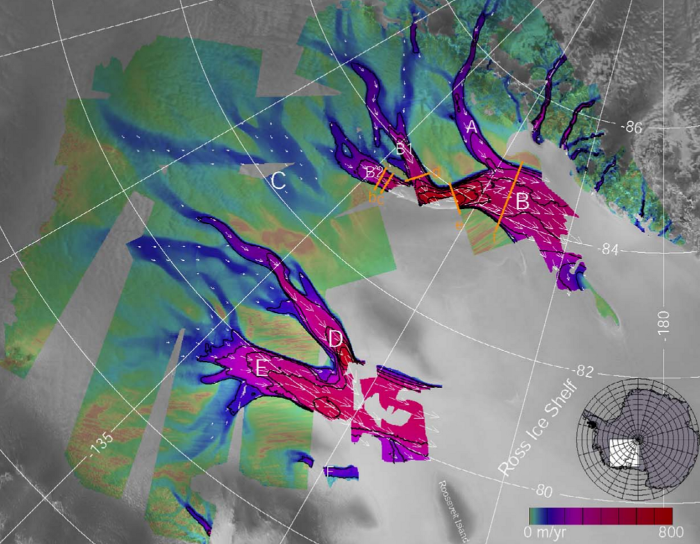
\includegraphics[width=\textwidth]{siple}

\vspace{0.3in}

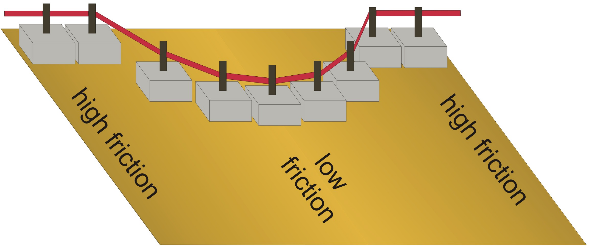
\includegraphics[width=1.1\textwidth]{schoof-sliders}
\end{column}
\end{columns}
\end{frame}


\begin{frame}
  \frametitle{SSA weak formulation}

\begin{itemize}
\item let $q = 1+\frac{1}{n}$ and $B = A^{1-q}$
\item suppose a basal yield stress distribution $\tau_c(x,y)$, zero on ice shelves
\item $2\,\Tnorm{\mathbf{V}}^2 := \sum_{i,j} (\mathbf{D}V_{ij})^2 + \sum_{i} (\mathbf{D}V_{ii})^2$
\item $\mathbf{F}$ denotes lateral force along calving front
\end{itemize}

\begin{block}{definition}
the horizontal velocity $\mathbf{U}\in W^{1,q}(\Omega)$ solves the coulomb friction SSA if it minimizes
\small
\begin{align*}
\mathcal{J}_{\text{SSA}}(\mathbf{V}) &= \int_\Omega \frac{2 B}{q} h \Tnorm{\mathbf{V}}^q + \rho g h \grad s \cdot \mathbf{V} + \tau_c |\mathbf{V}| - \int_{\partial\Omega} \mathbf{F} \cdot \mathbf{V}
\end{align*}
\end{block}

\end{frame}


\begin{frame}
  \frametitle{SSA weak formulation is well-posed}

\bigskip
\begin{block}{Theorem}
if $h\in L^\infty(\Omega)$ with $h\ge h_0>0$, and if $h |\grad s| \in L^{q/(q-1)}(\Omega)$, and if  $\tau_c \in L^{q/(q-1)}(\Omega)$, and as long as there is sufficient total basal resistance,$^\ast$ then the Coulomb friction SSA is well-posed problem for computing the velocity $\mathbf{U}\in W^{1,q}(\Omega)$ \hfill \scriptsize (Schoof, 2006)
\end{block}

\bigskip
\begin{itemize}
\item \emph{note}: because $\mathcal{J}_{\text{SSA}}$ is not differentiable, minimization on last slide is equivalent to a variational inequality but not to a PDE
\end{itemize}

\vfill
\scriptsize $\ast$: To stop the ice sheet from sliding whole into the sea.  There is a precise inequality.
\end{frame}

\begin{frame}
  \frametitle{marine ice sheets}

\begin{itemize}
\item marine ice sheets have all modes of flow
\item full of free boundaries
\item the Antarctic ice sheet is the marine ice sheet
\end{itemize}

\begin{center}
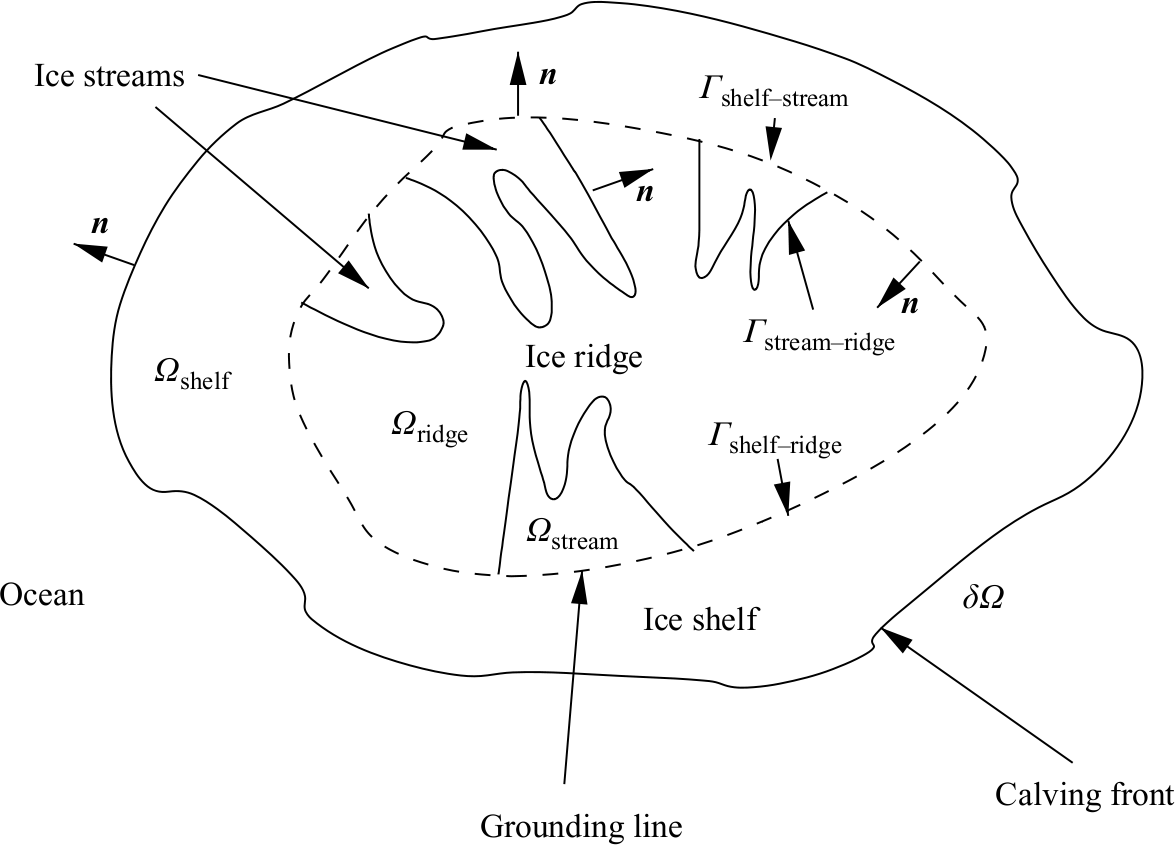
\includegraphics[width=0.7\textwidth]{schoof-planform}

\tiny cartoon from (Schoof, 2006)
\end{center}
\end{frame}


\begin{frame}
  \frametitle{ice sheet geometry evolution: set-up}

\begin{itemize}
\item recall $n\approx 3$ (i.e.~$n>1$):
  \begin{itemize}
  \item[$\circ$] $p = n+1 > 2$ \quad  is for SIA weak formulation
  \item[$\circ$] define $r = \frac{p-1}{2p}$; \quad SIA change of variables is $u=h^r$
  \item[$\circ$] $q = 1 + \frac{1}{n} < 2$ \quad  is for SSA weak formulation
  \end{itemize}
\item time-discretization $t_k$ with spacing $\tau_k = t_{k+1}-t_k$

\bigskip
\item time-dependent mass conservation: 
  $$\frac{\partial h}{\partial t} + \Div \left(  \int_b^s {\bf U}\, dz \right)  =  a$$
\item we hybridize: \hfill \scriptsize (Bueler \& Brown, 2009) \normalsize
  $$\mathbf{U} = \mathbf{U}_{\text{SIA}} + \mathbf{U}_{\text{SSA}}$$
\end{itemize}
\end{frame}


\begin{frame}
  \frametitle{ice sheet geometry evolution: a new algorithm}

\begin{enumerate}
\small
\item find velocity $\mathbf{U}_k \in \Wq$ that minimizes
\begin{align*}
\mathcal{J}_{\text{SSA}}(\mathbf{V}) &= \int_\Omega \frac{2 B}{q} h_k \Tnorm{\mathbf{V}}^q + \rho g h_k \grad s_k \cdot \mathbf{V} + \tau_c |\mathbf{V}| - \int_{\partial\Omega} \mathbf{F}_k \cdot \mathbf{V}
\end{align*}
\item find $h_{k+\frac12}$, the solution at $t_{k+1}$ of the advection problem:
$$\begin{cases}
  \frac{\partial h}{\partial t} + \Div \left(h\, \mathbf{U}_k\right) = 0, & t_k \le t \le t_{k+1}, \\
  h(t_k) = h_k. &
\end{cases}$$
\item transform: $u_{k+\frac12} = (h_{k+\frac12})^{1/r}$
\item find thickness $h_{k+1} = u^r$, i.e.~find $u\in\mathcal{K}$, that minimizes
\begin{align*}
\mathcal{J}_{\text{SIA}}(v) &= \int_{\Omega} \frac{1}{(r+1)\tau_k} v^{r+1} + \frac{\mu}{p} |\nabla v - \Phi(u_{k+\frac12})|^p - \left(\frac{1}{\tau_k} u_k^r + \alpha(u_{k+\frac12})\right) v
\end{align*}
\item repeat at {\color{dark blue} 1.} \hfill \scriptsize (Jouvet et al.~to appear)
\end{enumerate}
\end{frame}


\begin{frame}
  \frametitle{a quality of the SIA variational inequality} 

\begin{itemize}
\item every glaciologist believes this about steady climates:
	$$\text{if } a > 0 \text{ on a sub-domain } R \text{ then } s > b \text{ on } R$$
\item that is:
\begin{center}
 if it snows more than it melts then you get a glacier there
\end{center}
\end{itemize}

\begin{columns}
\begin{column}{0.6\textwidth}
\begin{itemize}
\small
\item uniformly-elliptic variational inequalities, e.g.~the classical obstacle problem,
\begin{align*}
\int_{\Omega}  \nabla u \cdot \nabla (v - u)  \ge  \int_{\Omega} f (v - u),
\end{align*}
for all $v\ge \psi$, do \emph{not} have the analogous property
\end{itemize}
\end{column}
\begin{column}{0.4\textwidth}
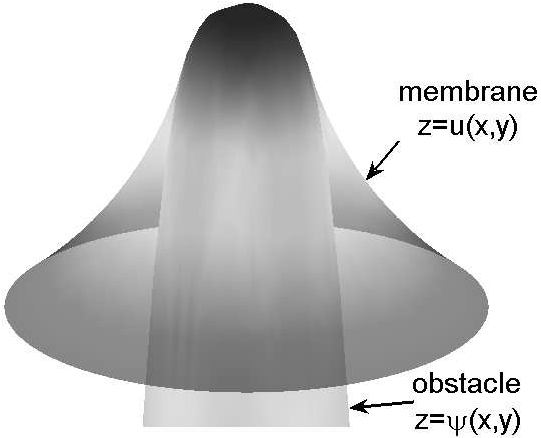
\includegraphics[width=\textwidth]{classicalobs}
\end{column}
\end{columns}
\end{frame}


\begin{frame}
  \frametitle{on TNNMG}

\small
to minimize a constrained or non-differentiable functional $\mathcal{J}$:
\begin{itemize}
\item let $I$ be the entire node index set, $\mathcal{I}=\mathcal{I}(v)$ the active set where $v$ is away from the obstacle/non-differentiability
\item let $\mathcal{F}:\RR^I \to \RR^I$ be a ``nonlinear Gauss-Seidel smoother'':
  \begin{itemize}
  \item[$\circ$]  gives correction that minimizes $\mathcal{J}$ at each node separately
  \item[$\circ$]  can be inexact
  \item[$\circ$]  the active set $\mathcal{I}$ can change
  \end{itemize}
\item let $\mathcal{D}$ be the domain of $\mathcal{J}$ and $\mathcal{P}_{\mathcal{D}}$ be a projection onto $\mathcal{D}$
\item then TNNMG generates sequence $u^l$ by:
\begin{align*}
  u^{l+\frac13} &= u^l + \mathcal{F}(u^l), \\
  u^{l+\frac23} &= u^{l+\frac13} - \left(\mathcal{J}''(u^{l+\frac13})_{\mathcal{I},\mathcal{I}}\right)^{-1} \mathcal{J}'(u^{l+\frac13})_{\mathcal{I}}, \\
  u^{l+1}       &= \operatorname{argmin}_{w,\rho\in[0,1]} \left\{\mathcal{J}(w) \big| w= \rho u^{l+\frac13} + (1-\rho) \mathcal{P}_{\mathcal{D}}(u^{l+\frac23}) \right\}
\end{align*}
\end{itemize}
\end{frame}

\end{document}
